\section{A Model of Chokepoint Bargaining}\label{sec:model}

The model has three players: Europe ($E$), the United States ($U$) and China ($C$). Europe decides whether ASML's most advanced tools, and the engineers who keep them running, reach Chinese fabs. We treat Europe as one actor and separate the Dutch licensing authority, the firm and the European Union in \cref{sec:decide}.

\subsection{Setup}\label{sec:setup}

\paragraph{Alignment.} Europe chooses an alignment $a\in\{A,X\}$. Under Atlantic alignment ($A$) ASML complies with US denial requirements. Exit ($X$) is a broad realignment of the chokepoint: Europe lets ASML sell and service EUV and advanced immersion DUV tools for Chinese fabs against US objection. Hedging, the continued sale and servicing of legacy immersion tools in China, has been the margin of dispute since 2023 (\cref{sec:record}); it is a secondary choice in \cref{prop:counter}(b). \Cref{sec:scope} states the scope conditions.

\paragraph{Stakes.} China gains $W>0$ from Europe's exit, of which a share $\theta\in[0,1]$ can be blocked by US jurisdiction over China-bound flows (the foreign direct product rule, de minimis rules and controls on US-made subsystems). That jurisdiction leaves ASML's supply to US-aligned fabs untouched, so we treat it as credible. The United States loses $V>0$ if Europe exits. $V$ is the patron's dependence on the chokepoint, what it gives up in the AI race when Chinese fabs gain access to ASML's frontier tools, and we measure it net of what flow jurisdiction still blocks: $V$ is Washington's loss from the share $1-\theta$ of access that exit would give. So $\theta$ scales both China's gain and Washington's loss.

\paragraph{Instruments and the baseline.} Washington's instruments $j$ are the core defence guarantee, force posture and enablers, access to frontier AI, and ASML's access to US inputs, persons and customers. After Europe chooses $a$, the United States sets each at a level $x_j(a)$ that is sequentially rational given its commitments, and Europe values it at $v_j(x_j)$. The conditional part of instrument $j$ is $d_j=v_j(x_j(A))-v_j(x_j(X))\ge 0$. The baseline is $x_j(A)$, Washington's ex post optimal provision to a loyal ally. A transfer is a promised increment above this baseline, and a threat is a withdrawal below it. Each instrument is thus counted once: frontier AI enters through $d_{ai}$, and only access beyond $x_{ai}(A)$ would be a transfer.

\subsection{Commitment}\label{sec:commitment}

One commitment technology governs every promise and every threat. Before Europe moves, each great power $i$ may attach a stake $m\le\bar m_i$ to any public conditional commitment, which it forfeits if the condition is met and it does not act. The stake is a reduced form for the audience costs of backing down, which tie hands rather than sink costs \citep{fearon1994domestic, fearon1997signaling}. The cap $\bar m_i$ applies to each commitment separately.

A promise to pay $\tau$ after Europe has moved has no ex post value to the promiser, so it is honoured if and only if $\tau\le\bar m_i$, and a threat whose execution costs the threatener $e$ ex post is credible if and only if $e\le\bar m_i$. Creating a stake costs nothing. A threat that deters is never carried out and costs its author nothing. One that is executed costs $e$, and $e\ge 0$ for every withdrawal from a loyal Europe because the baseline is Washington's ex post optimum.

Security uses the same technology: Washington can stake $m_S\le\bar m_U$ on a public threat to abandon a realigned Europe. Such a rule makes the guarantee less valuable to loyal allies before any crisis arrives, and that assurance cost (\cref{sec:conditionality}) makes conditionality an interior choice.

\subsection{Security, Other Instruments and the Exit Premium}\label{sec:security}

\paragraph{The core guarantee.} In a crisis, Washington defends Europe if its net stake in doing so exceeds a crisis-specific cost $\xi$, drawn from a continuous distribution $G$ with density $g$. Its stake in defending a realigned Europe is $s_X=s_0+s_B$, where $s_0$ is its own interest in European security and $s_B$ the value to it of European territory, airspace and bases. Its stake in defending a loyal Europe is $s_A=s_X+s_L$, where $s_L\ge 0$ is the added value of a loyal ally, for example Washington's reputation with other chokepoint holders. After exit, defending Europe also forfeits the stake $m_S$. The conditionality of the core guarantee is
\begin{equation}\label{eq:kappa}
\kappa=G(s_A)-G(s_X-m_S),\qquad s_A=s_X+s_L,\quad s_X=s_0+s_B,
\end{equation}
and its largest value, at $m_S=\bar m_U$, is $\bar\kappa=G(s_X+s_L)-G(s_X-\bar m_U)$. With $S_k$ Europe's crisis-weighted stake in core defence, the conditional part of the guarantee is $\kappa S_k$. Conditionality has two sources, the value of loyalty ($s_L$) and the staked threat of abandonment ($m_S$); Europe's dependence enters only through $S_k$.

\paragraph{Access and the silicon shield.} The term $s_B$ carries the access channel. A less committed United States ``may find itself relying on hefty cash payments to try to buy access'' \citep{carson2025allies}, so a Washington that needs such access has a reason to defend Europe whatever ASML does. If Washington would defend the territory on which ASML sits because it needs the firm, $s_B$ rises with $V$, a silicon shield. The shield is contested: writing about Taiwan, \citet{weil2025european} call the argument ``largely a hopeful narrative'', and we treat a rising $s_B(V)$ as an assumption. Its effect on conditionality has no fixed sign (\cref{prop:conditionality}(d)). Europe's own power to deny access is a hold-up instrument (\cref{sec:holdup}).

\paragraph{Posture and enablers.} Washington also provides a flow of posture and enablers: stationed forces, rotations, intelligence sharing, munitions and spare parts. The flow is cheap to adjust and can be withdrawn from one ally at a time, so it can be made conditional without touching the treaty commitment. Its conditional part is $d_p$.

\paragraph{The AI instrument.} Washington allocates frontier models, inference and advanced chips continuously, and the AI instrument's conditional part is $d_{ai}=v_{ai}(x_{ai}(A))-v_{ai}(x_{ai}(X))$. Scarce compute makes it cheap to cut an exiter's allocation, which raises $d_{ai}$. Scarcity could also lead Washington to ration loyal allies, which removes the conditional part only if they are cut to the exiter's level. Tiering loyal allies is itself costly: the AI Diffusion Rule of January 2025 tiered EU members and was set aside when BIS announced its rescission before the compliance date (\cref{sec:background}). We read the rescission as evidence that $d_{ai}$ stays positive when compute is scarce.

\paragraph{Firm-level penalties.} Washington can also penalize ASML itself, by entity listing or by denying US-origin inputs and US-person support for all of the firm's production. This costs Europe $f\ge 0$ and, by disrupting supply to US and allied fabs, harms the United States too. Washington's ex post gain from penalizing an exiting ASML is $\gamma-\varphi V$, where $\gamma\ge 0$ is the added denial benefit and $\varphi V$, with $\varphi>0$, the self-inflicted cost. The threat is credible if and only if its execution cost is within the cap, so
\[
d_f=\chi_f f,\qquad \chi_f=\mathbf 1\{\varphi V\le\gamma+\bar m_U\}.
\]
As in \citet{wolford2017alliances}, threats against a politically valuable ally lack credibility; here that applies only to penalties on the firm, and flow jurisdiction remains credible.

\paragraph{China's offer.} China can promise Europe a transfer if Europe exits: market access, credit, co-production or relief from its own export controls. A promise of $\tau_C$ costs China $\tau_C$, and Europe values it at $\lambda_C\tau_C$ with $\lambda_C\in(0,1]$, the lower value to Europe of what China offers in kind. China's promises are capped at $\bar m_C$. China may also value Washington's loss: with a relative-gains weight $\rho\ge 0$, the most it would pay for exit is $W_C=(1-\theta)W+\rho V$, and both terms shrink as $\theta$ rises. China's credible offer, in units of European utility, is
\begin{equation}\label{eq:omega}
\omega=\lambda_C\min\{W_C,\bar m_C\}.
\end{equation}
If the race is close to zero-sum, $\rho V$ is large and the cap binds; $\omega$ is then set by how far Europe trusts and values Chinese promises ($\lambda_C$ and $\bar m_C$).

\paragraph{Chinese punishment of alignment.} We set China's untargeted punishment of alignment to zero. Such a threat would be carried out whenever Europe aligned anyway, so China would make it only if punishing paid for itself, and it would then enter $Q$. China's observed coercion targets specific acts: informal sanctions after South Korea's THAAD deployment \citep{lim2022informal}, the 2025 Nexperia export ban after a Dutch order (\cref{sec:record}), and the listing of Japanese entities after Prime Minister Takaichi's statement on Taiwan (\cref{sec:cases}). We found no case in which China punished a holder for aligning its chokepoint controls with Washington. Chinese coercion therefore enters as counter-threats attached to particular concessions (\cref{prop:counter}) and to a transfer of control (\cref{sec:control}).

\paragraph{The exit premium.} Exit costs Europe the conditional parts of Washington's instruments plus an intrinsic cost $\eta\ge 0$, the value Europe places on keeping frontier capabilities from a rival that supports Russia's war:
\[
c=\kappa S_k+d_p+d_{ai}+d_f+\eta .
\]

\begin{definition}[Exit premium]\label{def:Q}
Europe's exit premium is China's credible offer net of the credible cost of exit,
\begin{equation}\label{eq:Q}
Q=\omega-c=\lambda_C\min\{(1-\theta)W+\rho V,\ \bar m_C\}-\kappa S_k-d_p-d_{ai}-\chi_f f-\eta .
\end{equation}
Europe's slack is $\Lambda=\pos{-Q}$.
\end{definition}

The premium follows \citet{hirschman1945national}, for whom a state's influence over a partner depends on what the partner would lose by leaving. Slack is the amount by which Europe's alternative to alignment falls short, in the sense of \citet{clayton2026putting} (\cref{sec:literature}). \Cref{tab:notation} collects the notation.

\begin{table}[t]
\centering
\small
\caption{Notation for the baseline model}\label{tab:notation}
\begin{tabularx}{\textwidth}{@{}l>{\raggedright\arraybackslash}Xl>{\raggedright\arraybackslash}X@{}}
\toprule
Symbol & Meaning & Symbol & Meaning\\
\midrule
$E,U,C$ & Europe, United States, China & $a\in\{A,X\}$ & Atlantic alignment or exit\\
$V$ & US loss from exit, net of flow jurisdiction (dependence) & $W$, $\theta$ & China's gain from exit; share blocked by US flow jurisdiction\\
$\rho$ & China's relative-gains weight & $W_C$ & most China would pay, $(1-\theta)W+\rho V$\\
$\bar m_U,\bar m_C$ & largest stake on one commitment & $\lambda_C$ & Europe's value of a unit of China's promise\\
$\omega$ & China's credible offer, \cref{eq:omega} & $x_j(a)$, $d_j$ & provision of instrument $j$; its conditional part\\
$s_0$, $s_B$ & US own interest in European security; access value & $s_L$ & added US value of a loyal ally\\
$s_A$, $s_X$ & US stake in defending a loyal, realigned Europe & $m_S$ & US stake on abandoning a realigned Europe\\
$G$, $g$ & distribution and density of crisis costs $\xi$ & $\kappa$, $\bar\kappa$ & conditionality of the core guarantee, \cref{eq:kappa}; its maximum\\
$S_k$ & Europe's crisis-weighted stake in core defence & $d_p$, $d_{ai}$ & conditional parts of posture and of the AI instrument\\
$f$, $\gamma$, $\varphi$ & firm penalty; US denial benefit; self-harm per unit of $V$ & $\chi_f$ & credibility of firm penalties\\
$\eta$ & Europe's intrinsic cost of exit & $c$ & credible cost of exit\\
$Q$ & exit premium, \cref{eq:Q} & $\Lambda$ & slack, $\pos{-Q}$\\
$\beta$ & Europe's probability of proposing & $\lambda$, $r$ & rupture hazard; discount rate\\
$\psi$ & rupture weight, $\lambda/(\lambda+r)$ & $P^*$ & equilibrium transfer flow to Europe\\
\bottomrule
\end{tabularx}
\end{table}

\paragraph{Timing.} \Cref{fig:timing} shows one period. The great powers announce conditional promises and threats and attach stakes. Washington and Beijing bid for Europe's alignment, and Europe chooses. Washington may then issue demands backed by its instruments (\cref{sec:slack}). Finally, instruments are used and rents paid, and each threat is carried out only if that is sequentially rational.

\begin{figure}[t]
\centering
\begin{tikzpicture}[x=1cm,y=1cm,font=\small]
\draw[-{Latex[length=2mm]}, line width=0.6pt, gray] (0,0) -- (14.2,0);
\foreach \x/\lab/\who in {0.8/{US offers $\tau_U\in[0,B_U]$}/{(1)}, 4.4/{China offers $\tau_C\in[0,B_C]$}/{(2)}, 8.0/{Europe chooses $A$ or $X$}/{(3)}, 11.6/{Instruments used}/{(4)}}{
  \fill[black] (\x,0) circle (2pt);
  \node[above=4pt, align=center, text width=3.1cm] at (\x,0) {\who\\ \lab};
}
\node[below=6pt, align=left, text width=5.2cm, font=\footnotesize] at (12.3,0) {US: defend in a crisis?\\ deny frontier AI? penalize ASML?\\ China: restrict critical inputs?};
\end{tikzpicture}
\caption{Timing of the static game. Each instrument in stage (4) is used only if doing so is sequentially rational (\cref{lem:credible}).}
\label{fig:timing}
\end{figure}


\subsection{The Bidding Benchmark}\label{sec:bidding}

In the benchmark, Washington and Beijing bid for Europe's alignment in an ascending auction, so either can raise its bid until neither wants to.

\begin{lemma}[Bidding benchmark]\label{lem:bidding}
Suppose the United States and China bid for Europe's alignment in an ascending (clock) auction in which bids are staked promises, Europe values China's promise $\tau_C$ at $\lambda_C\tau_C$, Europe chooses its alignment after the auction, and instruments are then used. Let $\bar z_U=\min\{V,\bar m_U\}$ and $Q=\lambda_C\min\{W_C,\bar m_C\}-c$.
\begin{enumerate}[label=(\roman*)]
\item After alignment $a$, the United States provides $x_j(a)$ for every instrument $j$, so exit lowers Europe's payoff, before transfers, by $c=\sum_j d_j+\eta$.
\item A promise of $\tau$ by power $i$ is honoured if and only if $\tau\le\bar m_i$. Bidding up to one's maximal credible bid (in units of Europe's payoff, $\bar z_U$ for the United States and $Q$ for China) is weakly dominant. In weakly undominated strategies, with an indifferent Europe aligning:
 \begin{enumerate}[label=(\alph*)]
 \item if $Q<V$ and $Q\le\bar m_U$, Europe aligns and the United States pays $\pos{Q}$;
 \item if $Q>\min\{V,\bar m_U\}$, Europe exits, and China's promise gives Europe $\min\{V,\bar m_U\}$ net of $c$.
 \end{enumerate}
 In both cases Europe's payoff is $\pos{\min\{Q,V,\bar m_U\}}$.
\item If $\bar m_U<Q<V$, every binding transfer $\tau\in[Q,V)$ from the United States to Europe would make both Europe and the United States strictly better off than the equilibrium (inefficient exit from limited US commitment).
\end{enumerate}
\end{lemma}

The losing bidder sets the price. The lemma restates known results (\cref{sec:literature}), and \citet[Supplement B.2]{clayton2026framework} derive a two-hegemon version. The weak-dominance argument is for the clock auction. In an alternating-raise auction (\cref{app:proofs}), subgame perfection alone does not pin down the price. Europe still aligns in every subgame-perfect equilibrium when $Q$ is more than one grid step below $\bar z_U$, and the price is within one grid step of $\pos{Q}$ when the losing bidder bids up to its maximal credible bid. What the lemma adds is the content of $Q$: China's bid enters Europe's participation constraint, and every cost of exit in $c$ is a conditional part that survives sequential rationality.\footnote{We value transfers at par. If delivering value $P$ to Europe costs Washington $a_U P$ with $a_U\le 1$, as for an exemption from an extraterritorial rule, then, when its commitment cap does not bind, Washington keeps Europe aligned if and only if $a_U Q<V$. Cheap in-kind transfers widen the range in which Washington wins without changing the price to Europe (\cref{sec:coding}).}

\subsection{Agenda Power and Rupture Risk}\label{sec:master}

We now give Europe a voice in the price by letting it bargain with Washington, with China's credible offer $\omega$, and hence $Q$, fixed and open to Europe as an exit option throughout. The two bargain over a perpetual signed transfer flow $P$: $P>0$ means Washington pays Europe and $P<0$ means Europe concedes. Agreements are binding.\footnote{Agreements are enforced by the stake technology of \cref{sec:commitment}. We assume that Washington's cap covers the agreed transfer ($\bar m_U\ge V$ suffices) and that a European concession is enforceable, for example because it is a policy Europe would have to reverse publicly.} Every $\Delta$ units of time, Europe proposes with probability $\beta\in[0,1)$ and Washington otherwise, and the responder accepts or rejects. After rejecting a US offer, Europe may exit, which yields flows $Q$ to Europe and $-V$ to Washington forever. If Europe does not exit, the dispute ruptures into exit with probability $\mu=1-e^{-\lambda\Delta}$, where $\lambda\ge 0$ is the rupture hazard; otherwise the status quo continues with flows $(0,0)$ and both discount at rate $r\ge 0$. Rupture is realignment that neither government chooses, for instance after a change of government in The Hague or an unintended escalation: a threat that leaves something to chance \citep{schelling1960strategy}. The disagreement point is the aligned status quo with no transfer, so $P$ replaces the bidding stage's payment. Write $\upsilon=e^{-(r+\lambda)\Delta}$ and $\psi_\Delta=\mu/(1-\upsilon)$, which tends to the rupture weight $\psi=\lambda/(\lambda+r)$ as $\Delta\to 0$.

\begin{proposition}[Bargaining with an outside option and rupture risk]\label{prop:master}
Let $Q<V$, $\beta\in[0,1)$, $r,\lambda\ge 0$ and $r+\lambda>0$.
\begin{enumerate}[label=(\roman*)]
\item For every $\Delta>0$, every subgame-perfect equilibrium gives Europe the same payoff $x^*(\Delta)$ and the United States $-x^*(\Delta)$ (closed forms in \cref{app:proofs}).
\item If $\lambda>0$, the subgame-perfect equilibrium is unique (up to Europe's exit choice at one point of indifference, which does not affect payoffs), and agreement is immediate. If $\lambda=0$, there are also stationary equilibria with delay, with the same payoffs.
\item As $\Delta\to 0$, $x^*(\Delta)$ and the equilibrium offer and demand converge to
\begin{equation}\label{eq:master}
P^*=\max\big\{Q,\ \psi\big(Q+\beta(V-Q)\big)\big\},\qquad \psi=\frac{\lambda}{\lambda+r}\in[0,1].
\end{equation}
If $r>0$, the second term is the larger one if and only if $Q<\hat Q\equiv\lambda\beta V/(r+\lambda\beta)$.
\end{enumerate}
\end{proposition}

Part (iii) describes bargaining in which offers come much faster than rupture or discounting. Europe's exit right is placed after it rejects a US offer.\footnote{If Europe could also exit right after Washington rejects Europe's own demand, the stationary equilibrium would have the same limit $P^*$, but when the outside option binds there would also be nonstationary equilibria in which Europe obtains up to $V$. Allowing exit only after Europe rejects a US offer pins down the outside-option principle \citep{binmore1989outside}. On the timing of outside options see \citet{shaked1994opting} and \citet{ponsati1998rubinstein}.} \Cref{fig:master} plots $P^*$ against $Q$ for three parameter sets.

\begin{figure}[t]
\centering
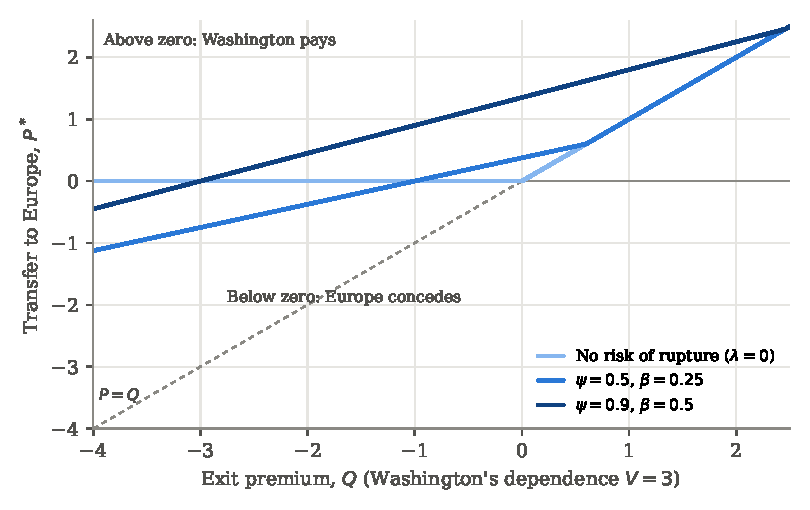
\includegraphics[width=0.8\textwidth]{figures/fig_master.pdf}
\caption{Equilibrium transfer to Europe under rupture risk (\cref{prop:master}) as a function of the exit premium, with $V=3$. Without rupture risk ($\lambda=0$) the transfer is $\pos{Q}$. With rupture weight $\psi=0.5$ and $\beta=0.25$, Washington pays Europe whenever $Q>-1$; with $\psi=0.9$ and $\beta=0.5$, whenever $Q>-3$. Below those values Europe concedes. Every curve lies on or above the dashed line $P=Q$ (\cref{cor:master}(a)).}
\label{fig:master}
\end{figure}

\begin{corollary}[Threshold and channels]\label{cor:master}
Under the conditions of \cref{prop:master}:
\begin{enumerate}[label=(\alph*)]
\item $P^*\ge Q$: Europe never concedes more than its slack, $-P^*\le\Lambda=\pos{-Q}$. (For $\Delta>0$ the value $x^*(\Delta)$ can be below $Q$, by at most $\beta(1-\upsilon)\pos{Q-\psi_\Delta V}/(1-\beta\upsilon)$.)
\item If $\lambda=0$, $P^*=\pos{Q}$; if $\beta=0$, $P^*=\max\{Q,\psi Q\}$. In either case $Q\le 0$ implies $P^*\le 0$.
\item $P^*>0$ if and only if $Q>0$, or $\lambda>0$ and $Q+\beta(V-Q)>0$.
\item Holding $Q$ fixed, $\partial P^*/\partial V=\beta\psi$ where the second term binds ($Q<\hat Q$) and $0$ where $Q>\hat Q$. If $Q$ itself depends on $V$, then $dP^*/dV=\psi[\beta+(1-\beta)\,dQ/dV]$ in the first case and $dQ/dV$ in the second.
\item $V$ enters $P^*$ directly only through the term $\beta\psi V$ (agenda power under rupture risk), and indirectly only through $Q$: through the rival's valuation, $\rho V$ in $W_C$ when $W_C<\bar m_C$ ($\partial\omega/\partial V=\lambda_C\rho$); through self-harming sanctions, $\chi_f=\mathbf 1\{\varphi V\le\gamma+\bar m_U\}$ (a rise in $V$ past $(\gamma+\bar m_U)/\varphi$ raises $Q$ by $f$); and through the silicon shield, $\kappa=G(s_X+s_L)-G(s_X-m_S)$ with $s_X=s_0+s_B(V)$ (which equals $\bar\kappa$ when $m_S=\bar m_U$), with a sign that depends on $g$. \Cref{prop:pain} adds the fifth channel, hold-up, which works through Washington's own need for ASML's servicing, not through $V$.
\end{enumerate}
Nesting: $\lambda=0$ gives $\pos{Q}$ (the outside-option principle); $r\to 0$ with $\lambda>0$ gives $Q+\beta(V-Q)$; $\beta=0$ gives $\max\{Q,\psi Q\}$ (Washington proposes); $\beta\to 1$ and $\lambda\to\infty$ give $V$.
\end{corollary}

The threshold in part (b) is the outside-option principle, and its substance is \citeauthor{wagner1988economic}'s (\cref{sec:literature}). Without rupture risk, a holder whose exit premium is negative gets nothing for its chokepoint, whoever proposes. $V$ then drops out because Europe lacks agenda power under rupture risk. A Europe that proposes in almost every round still cannot charge for $V$, since its only threat is exit and exit is credible only when $Q>0$. When $\lambda>0$, a rejected demand risks a rupture that costs Washington $V$, so Europe's demands carry weight in proportion to $\beta\psi$, a binary instance of the identity-dependent externalities through which a seller extracts surplus from parties that do not buy \citep{jehiel1996how}.

As $r\to 0$ the game becomes a random-proposer version of the breakdown model of \citet{binmore1986nash}. The corner $\beta\to 1$, $\lambda\to\infty$, in which Europe obtains all of $V$, is the bargaining implied when the summary of \citet{juijn2026europe} calls ASML ``the only card Europe still holds'' (\cref{sec:intro}). It requires take-it-or-leave-it demands whose rejection ends in realignment with near certainty, a commitment Europe has not shown it can make.

Rupture risk cuts both ways. When $Q<0$, a rupture would leave Europe worse off than the aligned status quo, and Washington can extract part of the value to Europe of avoiding it: $P^*<0$ if and only if $\lambda>0$ and $Q+\beta(V-Q)<0$. By \cref{cor:master}(a), though, Europe never concedes more than its slack. \Cref{sec:slack} shows that in the bidding benchmark slack also caps what Washington obtains by any combination of conditional threats. \Cref{rem:rupture} extends the cap to rupture risk.
